\section{Investigación previa}

\subsection{Qué es y cómo funciona la transmisión y recepción con Amplitud Modulada (AM)}
La modulación AM es una técnica de transmisión de datos que basa su funcionamiento en encriptación de información como modificaciones 
de amplitud de ondas de radio.
 
La modulación es el proceso en el cual se combina una señal de baja frecuencia (información) con una portadora de alta frecuencia para 
que pueda ser transmitida. Es así como se toma una señal portadora y se modifica su amplitud en base a las variaciones de la onda que se desea enviar. Esto da como resultado la misma onda portadora, pero con variaciones de amplitud en sus extremos superiores e inferiores que contienen la información.

Es así como la transmisión de información involucra la generación de una onda portadora, la modulación de la información en esta 
portadora, la eventual amplificación de esta señal y por último la transmisión de la onda a través de una antena.

En contraposición, la modulación es el proceso de extraer la señal moduladora de la señal portadora. Este ejercicio puede abordarse de 
diversas formas, pero aquí trataremos con la de detección de envolvente. Este método es utilizado cuando trabajamos con señales con un 
índice de modulación m=<1 y consiste en rectificar un la onda de entrada, dejando solo el lado positivo y luego seguir la envolvente de 
la portadora, que efectivamente corresponde a la señal moduladora original.

De este modo, la recepción de una señal consiste en recibir una onda a través de una antena, rectificar usualmente a valores solo 
positivos, para finalmente filtrar para eliminar los elementos de alta frecuencia comúnmente de la portadora, dejando así una salida 
que corresponde a la señal moduladora original.


El índice de modulación es una medida de la variación de la amplitud de la onda portadora. Visto de otro modo, se ve como la variación 
introducida en una portadora por la modulación y se define como $m = \frac{A_m}{A_c}$, donde $A_m$ es la amplitud de la señal de 
modulación y $A_c$ la amplitud de la señal portadora. Dada la razón m siempre tomará valores positivos o 0, donde: $m=0$ equivale a una 
portadora no modulada o una moduladora sin información. $0<m<1$ equivale a una portadora submodulada. Esto quiere decir que no se utilizó 
el total de la portadora para modular, pero sus consecuencias no son tan significativas más allá de un desaprovechamiento de potencial. 
$m=1$ equivale a una modulación ideal, donde se utiliza todo el potencial de la portadora, variando su amplitud desde su máximo hasta 0. 
Finalmente $m>1$ es una portadora sobremodulada, lo que resulta problemático dado que hay puntos en que la amplitud de la moduladora se 
invierte, dando una envolvente invertida la que es difícil de demodular e introduciendo distorsiones en la señal que se quiere 
transmitir.


\begin{figure}[h!]
    \centering
    \includegraphics[width=0.75\linewidth]{img/transisor.jpg}
    \caption{Diagrama de Bode para Filtro Pasabajos}
    \label{fig:bode_butter}
\end{figure}

\begin{figure}[h!]
    \centering
    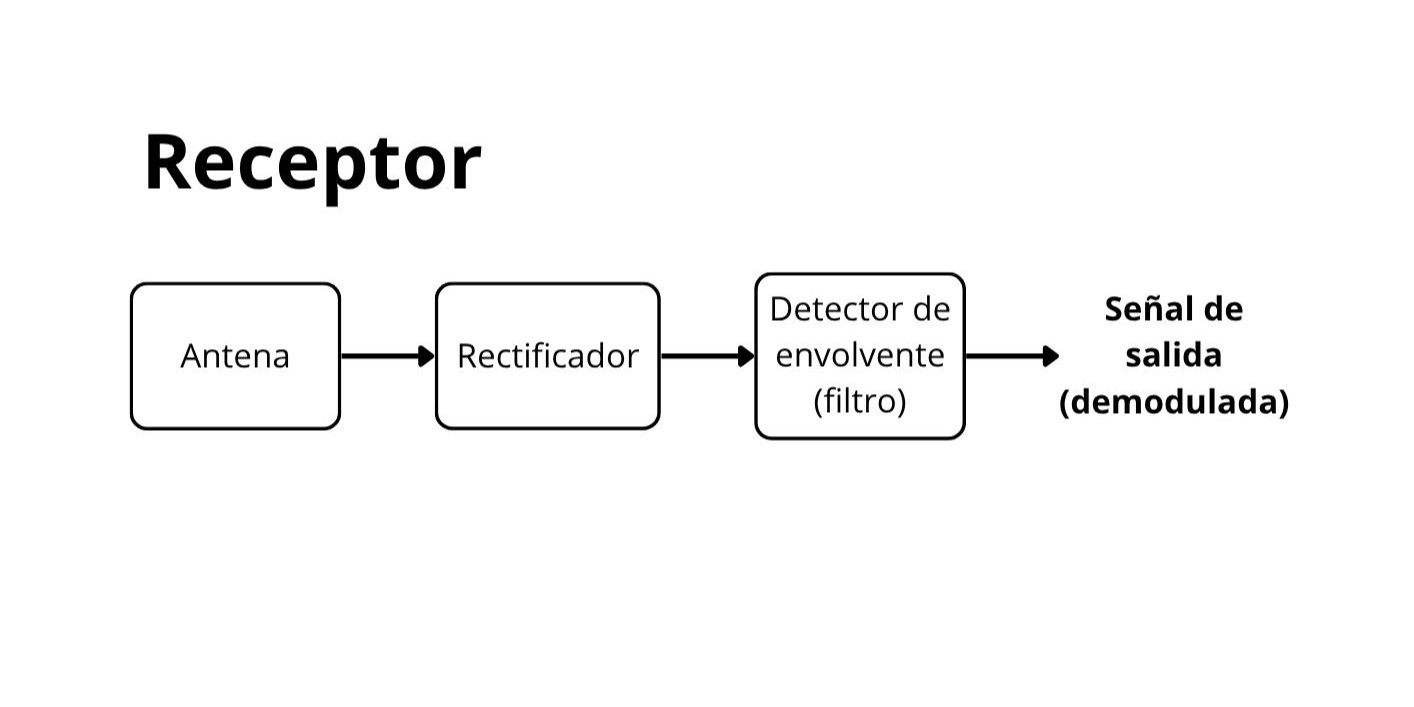
\includegraphics[width=0.75\linewidth]{img/receptor.jpg}
    \caption{Diagrama de Bode para Filtro Pasabajos}
    \label{fig:bode_butter}
\end{figure}
